\chapter{Adding Memory to the Agents}
\section{Overview}
Until now, we have assumed that all of the problems are fully observable, which means that they follow an MDP. The assumption behind this is that using the information given by the observation of the environment should be sufficient to fully understand its state. Thus:

\begin{equation}
    o_{t} = s_{t}
\end{equation}

But this is not always true and D-COACH is not suited to perform well in POMDPs. There are different reasons of why a problem is partially observed. In this work we focus on those cases where the observations represent instant information sensed from the environment but the state is described by time-dependent phenomena. For instance, if we want to estimate the velocity of a flying drone using information obtained from an RGB camera, it is necessary to combine data from different time steps in order to achieve this. 

In this chapter we aim to use a function approximation model that adds memory to the agents and to propose a variation of D-COACH which is capable of training this model. The idea is to validate this approach through simulations, establishing a baseline for further research in memory-based deep interactive learning.

\section{Method}
There are two well-known approaches for adding memory to agents in sequential decision-making problems when using DNNs as function approximator:

\begin{enumerate}
    \item \textbf{Observation stacking:} This approach consists of stacking a fixed number of past observations to the current one and using this modified observation as the input of the policy. 
    \item \textbf{Recurrent models:} This approach consists of using policies based on RNNs. Given that these models have an internal state, they can store information from the past (i.e. they have memory) and use it in posterior inferences. 
\end{enumerate}

One of the main issues of observation stacking is that the memory of this model is determined by the number of stacked observations. In high-dimensional state problems, the size of the input can increase considerably as the number of stacked observations increment, producing an overhead that makes these approaches impractical. 

On the other hand, in RNNs the overhead is determined by the size of its hidden layers and the size of the sequences used when updating the weights of the model. As a consequence, the most important overhead of RNNs occurs when training. Nevertheless, several DRL approaches have used this approach without reporting large overheads.

Given the more practical usage of recurrent models, in this work we use RNNs policies to test the viability of D-COACH for solving POMDPs. 

\subsection{Learning to Remember}

\section{Low-dimensional State with Memory}


\section{High-dimensional State with Memory}

\section{Experiments and Results}

\begin{figure}[h]
    \centering
    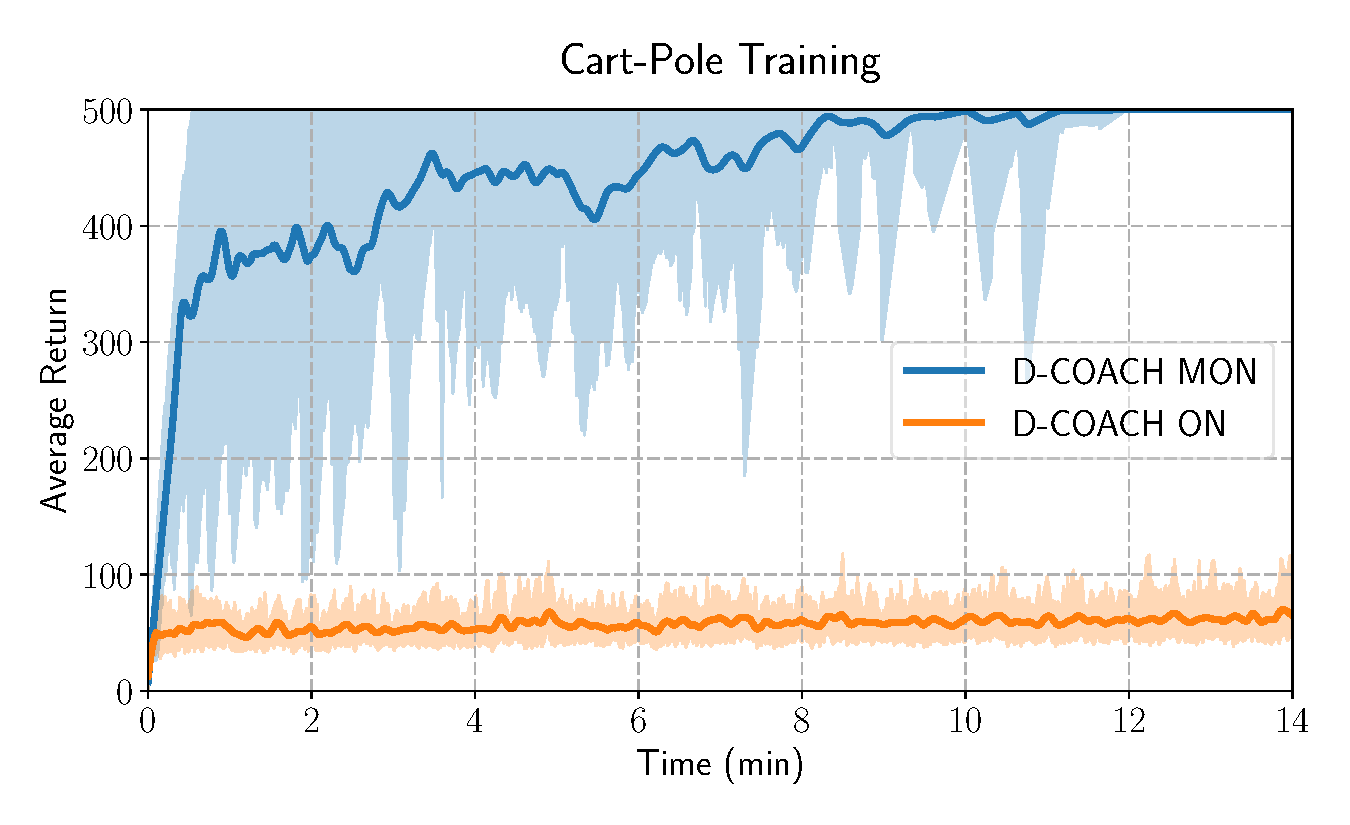
\includegraphics[width=0.9\linewidth]{imagenes/cap3/cartpole_LD_model.pdf}
    \caption{Evolution of the error while learning the reacher task. }
    \label{fig:reacher_exp}
\end{figure}

\begin{figure}[h]
    \centering
    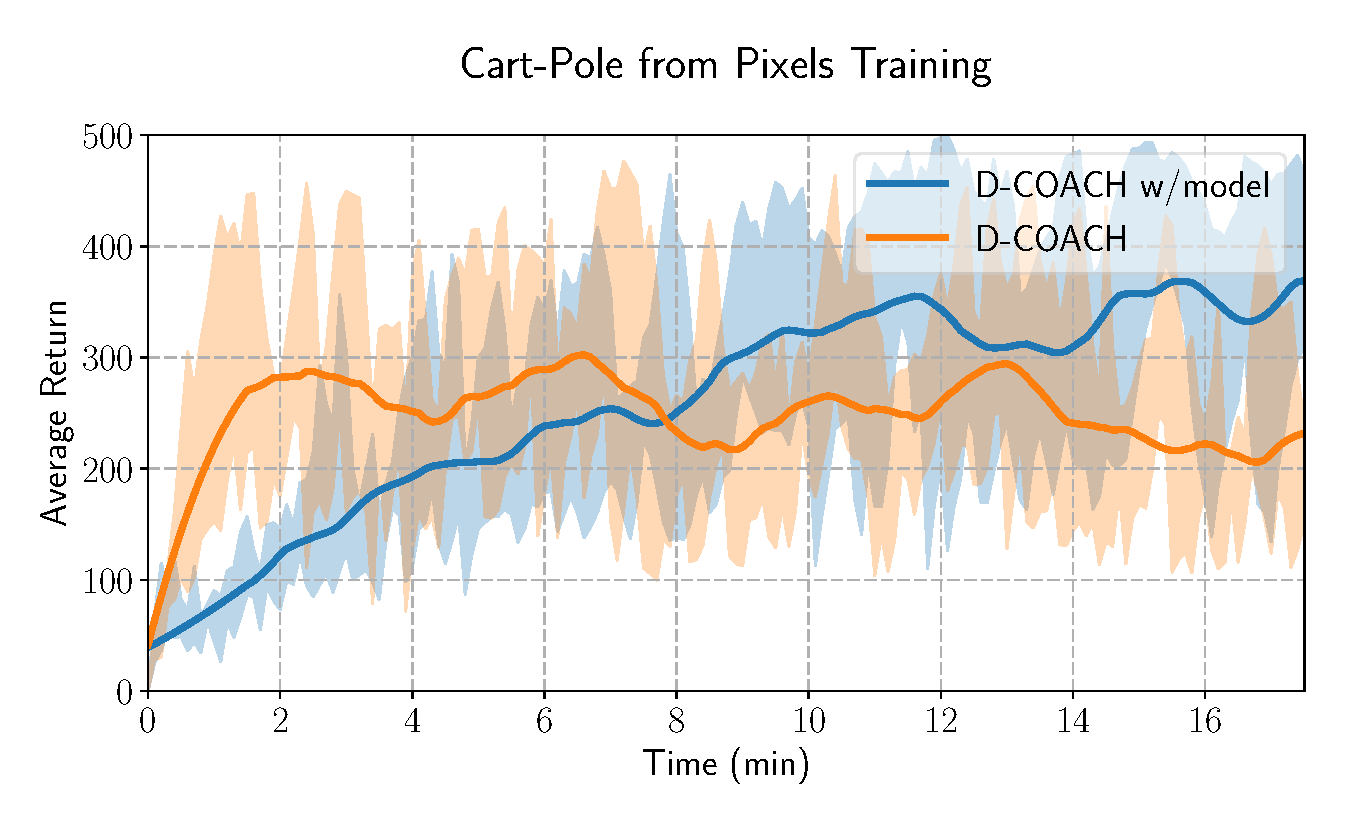
\includegraphics[width=0.9\linewidth]{imagenes/cap3/cartpole_HD_model.pdf}
    \caption{Evolution of the error while learning the reacher task. }
    \label{fig:reacher_exp}
\end{figure}


\begin{figure}[h]
    \centering
    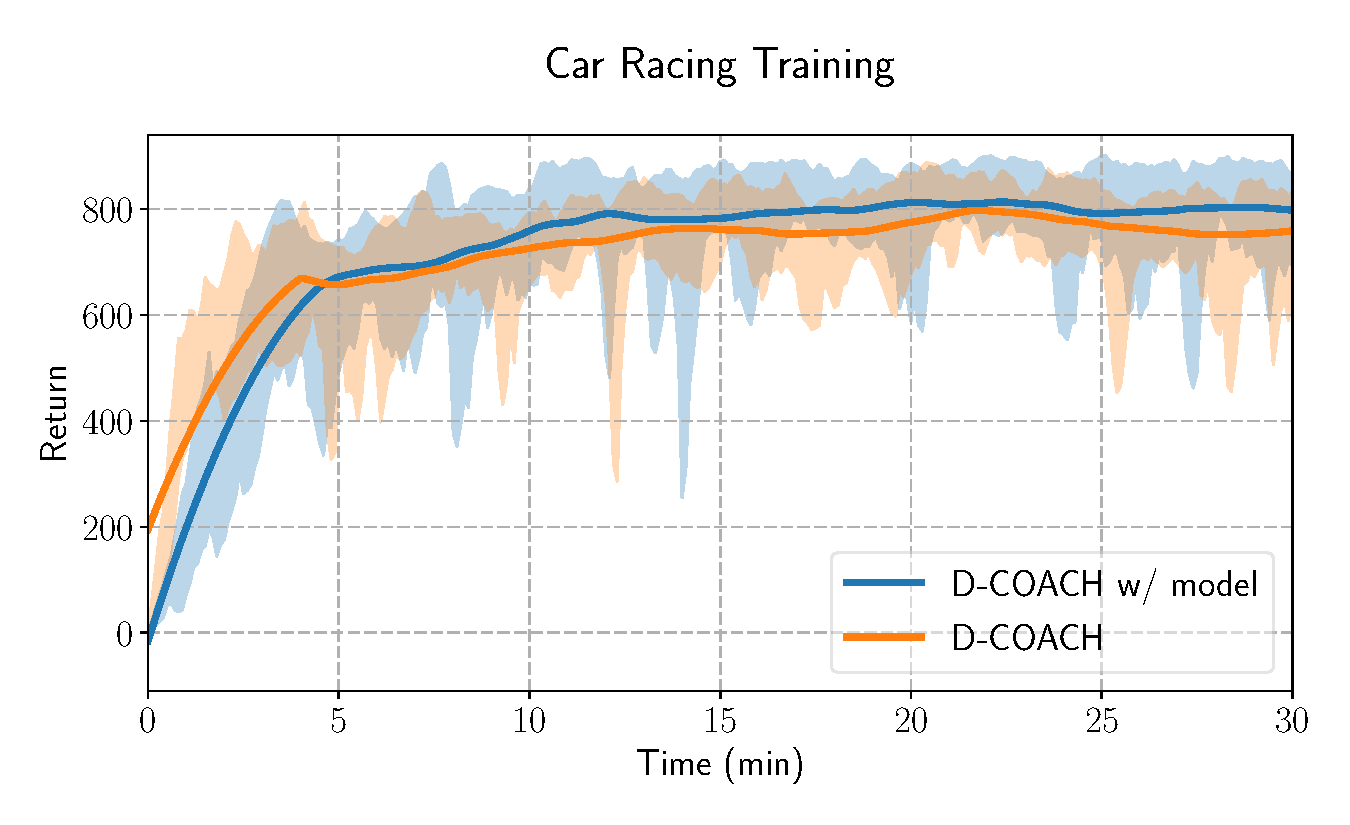
\includegraphics[width=0.9\linewidth]{imagenes/cap3/car_racing_lstm.pdf}
    \caption{Evolution of the error while learning the reacher task. }
    \label{fig:reacher_exp}
\end{figure}